% Centri — Weekly progress (week ending 2026-06-30)
% Compile: pdflatex -interaction=nonstopmode centri-weekly-2026-06-30.tex   (run twice)
\documentclass[aspectratio=169,10pt]{beamer}
\usetheme{metropolis}
\metroset{sectionpage=progressbar, subsectionpage=none, numbering=fraction, progressbar=frametitle}

\usepackage{booktabs}
\usepackage{amsmath,amssymb}
\usepackage{siunitx}
\usepackage{xcolor}
\usepackage{colortbl}
\usepackage{graphicx}
\graphicspath{{figs/}}
\usepackage{tikz}
\usetikzlibrary{arrows.meta,positioning,calc,shapes.geometric,fit,backgrounds}
\usepackage[most]{tcolorbox}

% ---- palette (shared with the other Centri decks) ------------------------
\definecolor{cMeas}{HTML}{1F6FB2}
\definecolor{cPed}{HTML}{B5651D}
\definecolor{cApp}{HTML}{2E7D32}
\definecolor{cInfra}{HTML}{5E35B1}
\definecolor{cAccent}{HTML}{C62828}
\definecolor{cGrey}{HTML}{616161}
\definecolor{cBg}{HTML}{F4F6F8}
% per-tier accents, matching the rendered PDFs (basic green / int blue / adv purple)
\definecolor{cBasic}{HTML}{2E7D32}
\definecolor{cInter}{HTML}{1565C0}
\definecolor{cAdv}{HTML}{6A1B9A}
\definecolor{cExp}{HTML}{00695C}   % planned 4th tier (Evaluate--Create)
\setbeamercolor{frametitle}{bg=cMeas}
\setbeamercolor{progress bar}{fg=cAccent}

\newcommand{\hl}[1]{{\bfseries\color{cAccent}#1}}
\newcommand{\ok}{{\color{cApp}\textbf{\checkmark}}}

\tikzset{
  box/.style={rounded corners=2pt, draw=#1, line width=0.8pt, fill=#1!8,
              text=black, align=center, font=\scriptsize, inner sep=4pt, minimum height=8mm},
  node distance=5mm and 8mm,
  flow/.style={-{Stealth[length=2.2mm]}, line width=0.7pt, draw=cGrey},
}

\title{Centri --- Weekly Progress}
\subtitle{Difficulty-tiered learning material: theory, pipeline, and evaluation}
\author{Damar Albaribin}
\institute{MSc Thesis --- advisor: Prof.\ Wu-Yuin Hwang}
\date{Week ending 2026-06-30}

\begin{document}
\maketitle

% =========================================================================
\begin{frame}{Where this came from --- and what this week delivered}
\small
\begin{tcolorbox}[colback=cGrey!8,colframe=cGrey,title=\footnotesize Context --- two inputs,boxsep=2pt,left=4pt,right=4pt]
\scriptsize
\textbf{\texttt{note-29}:} one video $\rightarrow$ \textbf{3 learning materials} (basic / intermediate /
advanced); evaluate each $\rightarrow$ a per-tier F1. \emph{Hypothesised:} basic \emph{high} (easy text
overlaps), advanced \emph{lowest} (unique). \emph{To do:} ground the definitions in literature.\\[2pt]
\textbf{Prof's note (2 weeks ago):} value-first, authentic scenes (5W$+$1H, daily life); relationships
\emph{through annotation}; multimodal BERTScore (caption then score); scale-up to 10--15 phenomena /
$\sim$30 videos; and a \textbf{knowledge graph of easy/medium/hard understanding} (Paper 2)
--- which motivates these difficulty tiers.
\end{tcolorbox}
\vspace{0.2em}
This week turned the tiered-material direction into a real, validated feature:
\begin{itemize}\setlength\itemsep{1pt}
  \item \textbf{\color{cMeas}Wired into the live pipeline} \ok\ --- a seeded step produces the 3 tiers,
  each with its own PDF; grounded in \textbf{Bloom + Cognitive Load Theory} (the literature note-29 asked for).
  \item \textbf{\color{cPed}A grounding gate} \ok\ --- checks the physics computes; \hl{caught 2 already-shipped
  materials with wrong arithmetic}, now fixed.
  \item \textbf{\color{cApp}Difficulty measured, not asserted} \ok\ --- and the F1 hypothesis was
  \hl{overturned}: basic scores \emph{lowest}, not highest (evaluation slides).
\end{itemize}
{\footnotesize Run end-to-end for \textbf{all 5 objects} (15 tiers); packaged for evaluation. Nothing committed yet.}
\end{frame}

% =========================================================================
\section{How we define difficulty --- the theory}

\begin{frame}{The theory: two lenses that must agree}
\small
A learner \emph{reads} the material --- it asks them to do nothing --- so we cannot define
difficulty by a task verb. We define it with two established theories:
\vspace{0.4em}
\begin{columns}[T]
\begin{column}{0.5\textwidth}
\begin{tcolorbox}[colback=cMeas!6,colframe=cMeas,title=\footnotesize Cognitive Load Theory,boxsep=2pt,left=3pt,right=3pt]
\scriptsize Sweller (1994, 2010) --- \textbf{element interactivity}: how many quantities,
relations, and time-states the passage integrates \emph{at once}. The primary lever for
exposition. More interacting elements held simultaneously $=$ higher intrinsic load.
\end{tcolorbox}
\end{column}
\begin{column}{0.5\textwidth}
\begin{tcolorbox}[colback=cPed!6,colframe=cPed,title=\footnotesize Bloom's Revised Taxonomy,boxsep=2pt,left=3pt,right=3pt]
\scriptsize Anderson \& Krathwohl (2001) --- the cognitive \textbf{objective} the passage
\emph{equips the reader to reach} (Remember $\rightarrow$ Understand $\rightarrow$ Apply
$\rightarrow$ Analyze $\rightarrow$ Evaluate). A target outcome, \emph{not} task verbs in the text.
\end{tcolorbox}
\end{column}
\end{columns}
\vspace{0.6em}
\begin{center}
\begin{tcolorbox}[colback=cAccent!6,colframe=cAccent,boxsep=2pt,left=5pt,right=5pt,width=0.92\textwidth]
\centering\small \textbf{Difficulty} $=$ (how many interacting elements the passage integrates,
\textit{CLT}) $\times$ (the cognitive objective it builds toward, \textit{Bloom}).\\
{\scriptsize Both must point to the same tier --- if they disagree, the material is mis-designed and is rewritten.}
\end{tcolorbox}
\end{center}
\end{frame}

\begin{frame}{The depth ladder is the measurement seed itself}
\scriptsize
Each tier is defined by \textbf{which ground-truth seed fields it may draw on} --- this is what
makes the tiers reproducible instead of subjective. Numbers always come only from the seed.
\vspace{0.3em}
\renewcommand{\arraystretch}{1.25}
\begin{tabular}{@{}p{1.6cm}p{4.3cm}p{2.2cm}p{2.6cm}@{}}
\toprule
\textbf{Tier} & \textbf{Seed fields used} & \textbf{CLT load} & \textbf{Bloom objective} \\
\midrule
\rowcolor{cBasic!10}\textbf{\color{cBasic}Basic} & radius + the \emph{idea} of an inward pull;
no equations, words only & low --- one idea at a time & Remember / Understand \\
\rowcolor{cInter!10}\textbf{\color{cInter}Intermediate} & $+\ \omega, v, a_c, T, f$ with values
$+$ the relations $v{=}\omega r$, $a_c{=}\omega^2 r$, $T{=}2\pi/\omega$ & moderate --- a handful
of interacting variables & Apply / Analyze \\
\rowcolor{cAdv!10}\textbf{\color{cAdv}Advanced} & $+\ \alpha$, the spin-up/coast-down timeline,
$a_c \propto \omega^2$, the scale caveat & high --- many quantities, over time, with limits &
Analyze / Evaluate \\
\bottomrule
\end{tabular}
\vspace{0.5em}

{\footnotesize The figures are tiered too (basic 2 / intermediate 3 + core table / advanced 5 +
full table) so the \emph{visual} load matches the prose --- a one-idea passage is not printed next
to a quadratic $a_c(t)$ curve. Spec: \texttt{docs/difficulty-tiered-material-spec.md}.}
\end{frame}

% =========================================================================
\section{Wired into the live pipeline}

\begin{frame}{From seed to three grounded materials --- with a gate}
\scriptsize
\begin{center}
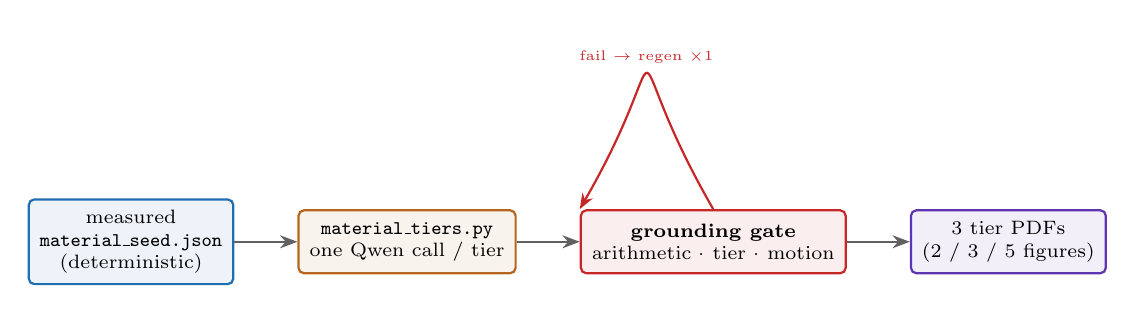
\begin{tikzpicture}
\node[box=cMeas] (seed) {measured\\\texttt{material\_seed.json}\\(deterministic)};
\node[box=cPed, right=of seed] (gen) {\texttt{material\_tiers.py}\\one Qwen call / tier};
\node[box=cAccent, right=of gen] (gate) {\textbf{grounding gate}\\arithmetic · tier · motion};
\node[box=cInfra, right=of gate] (pdf) {3 tier PDFs\\(2 / 3 / 5 figures)};
\draw[flow] (seed)--(gen); \draw[flow] (gen)--(gate); \draw[flow] (gate)--(pdf);
\draw[-{Stealth[length=2mm]}, line width=0.8pt, draw=cAccent] (gate.north) to[out=120,in=60,looseness=4] node[above,font=\tiny,text=cAccent]{fail $\rightarrow$ regen $\times1$} (gate.north west);
\end{tikzpicture}
\end{center}
\vspace{0.2em}
\begin{itemize}\setlength\itemsep{2pt}
  \item New seeded step \texttt{python -m analysis.material\_tiers} --- reads the seed, writes
  \texttt{material.\{basic,intermediate,advanced\}.json}; one local-Qwen call per tier (an A3B
  model bleeds vocabulary if asked for all three at once).
  \item The renderer emits \textbf{one PDF pair per tier}, each with a difficulty-matched figure
  set and a per-tier colour + level badge. Orchestrator + LaTeX gate updated to match.
  \item \textbf{Run end-to-end in the real worker for all 5 objects} (15 tiers): each tier $\rightarrow$
  render $\rightarrow$ compile, PDFs of \textbf{3 / 4 / 7 pages} and \textbf{4 / 6 / 9 figures} --- visual
  load scales with tier. Gate: \textbf{all passed}; full verifier \textbf{15/15 grounded}.
\end{itemize}
\end{frame}

% =========================================================================
\section{The grounding gate --- and what it caught}

\begin{frame}{BERTScore is blind to whether the physics computes}
\small
We added a deterministic, model-free verifier that checks every material against the measured
ground truth (the seed): \textbf{arithmetic closure}, number-grounding, tier compliance,
motion-type faithfulness. It is now a \hl{pre-ship gate} inside the tier step.
\vspace{0.4em}
\begin{tcolorbox}[colback=cAccent!6,colframe=cAccent,title=\footnotesize It found 2 of 5 already-shipped materials had wrong arithmetic,boxsep=2pt]
\scriptsize
Bicycle and turntable: the old single-material generator plugged the \emph{time-averaged} mean
$\omega$ into $a_c=\omega^2 r$ and $T=2\pi/\omega$ --- which do \emph{not} close for non-uniform
motion (Jensen's inequality: $\text{mean}(\omega^2) > (\text{mean }\omega)^2$).
E.g.\ stated $a_c = 3.99$, actually computes to $3.50$.
\end{tcolorbox}
\vspace{0.3em}
\textbf{Fixed at the source:} the seed now reports the fitted radius and instructs the model to
verify every identity at a \emph{single timeline instant} (where $v=\omega r$ and $a_c=\omega^2 r$
close exactly). Both materials regenerated $\rightarrow$ \textbf{pass}; PDFs re-rendered;
the evaluation export refreshed (all 5 grounded; relevance unchanged at \textbf{F1 $0.840\pm0.010$}).
\end{frame}

% =========================================================================
\section{Evaluation --- the ladder is now measured}

\begin{frame}{Per-tier relevance vs.\ an independent difficulty signal}
\scriptsize
All \textbf{5 objects $\times$ 3 tiers} (n$=$15). \emph{Relevance} = BERTScore, scored both against the
section-aligned OpenStax §6.2 gold \textbf{and} the full English reference set (19 refs). \emph{Difficulty}
= a model-free signal (\texttt{grade\_material\_difficulty.py}): Flesch readability + an element-interactivity
count (CLT proxy). Mean $\pm$ SD across objects.
\vspace{0.3em}
\renewcommand{\arraystretch}{1.25}
\begin{columns}[T]
\begin{column}{0.49\textwidth}
\centering {\scriptsize\bfseries Relevance (BERTScore F1)}\\[2pt]
\begin{tabular}{@{}lcc@{}}
\toprule
\textbf{Tier} & \textbf{vs §6.2} & \textbf{vs 19-ref set} \\
\midrule
\rowcolor{cBasic!10}\textbf{\color{cBasic}basic} & 0.811 & 0.798 \\
\rowcolor{cInter!10}\textbf{\color{cInter}interm.} & 0.831 & 0.806 \\
\rowcolor{cAdv!10}\textbf{\color{cAdv}advanced} & 0.828 & 0.800 \\
\bottomrule
\end{tabular}
\end{column}
\begin{column}{0.49\textwidth}
\centering {\scriptsize\bfseries Difficulty (independent)}\\[2pt]
\begin{tabular}{@{}lcccc@{}}
\toprule
\textbf{Tier} & \textbf{ease} & \textbf{FK grade} & {\color{cGrey}\textbf{Bloom}} & \textbf{EI} \\
 & {\tiny easier$\uparrow$} & {\tiny harder$\uparrow$} & {\tiny\color{cGrey} planned} & {\tiny CLT} \\
\midrule
\rowcolor{cBasic!10}\textbf{\color{cBasic}basic} & 68.0 & 7.1 & {\color{cGrey}--} & 3 \\
\rowcolor{cInter!10}\textbf{\color{cInter}interm.} & 52.3 & 8.3 & {\color{cGrey}--} & 28 \\
\rowcolor{cAdv!10}\textbf{\color{cAdv}advanced} & 37.0 & 10.9 & {\color{cGrey}--} & 23 \\
\bottomrule
\end{tabular}
\end{column}
\end{columns}
\vspace{0.4em}
\textbf{\color{cApp}Readability rises monotonically for all 5 objects}; relevance ranking is stable across
all 19 references (§6.2 is not cherry-picked). The tiers are \emph{real}, not just labelled.
{\footnotesize\ (EI count saturates between intermediate$\leftrightarrow$advanced --- advanced trades
\emph{breadth} of quantities for \emph{depth}, which FK grade captures and a raw count does not.)}
\vspace{0.3em}
\begin{tcolorbox}[colback=cGrey!8,colframe=cGrey,boxsep=1pt,left=4pt,right=4pt]
\tiny \textbf{Planned (next):} fill the \textbf{Bloom level} column of the independent difficulty
signal (placed between FK grade and EI: surface $\rightarrow$ objective $\rightarrow$ structure) ---
Bloom objective \emph{assessed} per material (LLM-judge / rater), so the achieved level can be checked
against the designed one (the ``two lenses must agree'' test, now measured). Also considering a
\textbf{4th tier} (Evaluate$\rightarrow$Create: design-your-own-experiment / error analysis) with its
own colour \textcolor{cExp}{$\blacksquare$}, extending the ladder to four points.
\end{tcolorbox}
\end{frame}

\begin{frame}{The key methodological finding}
\small
\begin{tcolorbox}[colback=cMeas!6,colframe=cMeas,boxsep=2pt,left=5pt,right=5pt]
BERTScore against a fixed reference does \textbf{not} track difficulty the way \texttt{note-29}
hypothesised. \hl{Basic scores \emph{lowest} on every one of the 5 objects} --- because it has the
fewest equation-like elements (interactivity $\approx$3) and therefore the least lexical overlap with the
equation-dense textbook. The pattern holds against all 19 references, not just §6.2.
\end{tcolorbox}
\vspace{0.5em}
\begin{itemize}\setlength\itemsep{3pt}
  \item So BERTScore-vs-reference measures \textbf{element / lexical density, not pedagogical
  quality}. The independent signal makes this visible: lowest interactivity \emph{and} lowest F1
  are the same tier, robustly at n$=$5.
  \item This is exactly why we built the \textbf{grounding verifier} --- and why the real quality
  axes still to come (LLM-as-judge, teacher panel) matter.
  \item Honest test of the \texttt{note-29} hypothesis needs \textbf{tier-matched references} --- a
  single fixed reference cannot do it.
\end{itemize}
\end{frame}

% =========================================================================
\section{Scaling to new phenomena --- the measurement side}

\begin{frame}{New capture batch: four phenomena, selected by data quality}
\scriptsize
Toward the advisor's \emph{scale-up} ask, a new batch (16 clips) adds \textbf{four distinct
centripetal phenomena}. Each clip is scored by \textbf{tracking data quality}; the best per
phenomenon is run. Identical blades/spokes alias appearance trackers, so the mode is chosen per
scene --- local \textbf{colour}/\textbf{frequency} where a marker or blade-pass works, \textbf{SAM3}
object-tracking where it wins. Every trajectory is pre-computed and \hl{cache-seeded for the agent}
(cache-HIT), and \textbf{all five ran end-to-end} $\rightarrow$ 3 tier PDFs each.
\vspace{0.3em}
\renewcommand{\arraystretch}{1.1}
\begin{center}
\begin{tabular}{@{}p{3.15cm}p{1.2cm}p{2.35cm}p{2.75cm}c@{}}
\toprule
\textbf{Phenomenon} & \textbf{Clip} & \textbf{Tracking mode} & \textbf{Data quality} & \\
\midrule
Ceiling fan (5 blades, red mark) & 4027, 4028 & frequency (blade-pass FFT) & clean $\omega(t)$, hop-immune & \ok \\
Computer fan (11 blades, red mark) & 4029 & colour (red marker) & 87\% cov, CV 0.07 & \ok \\
Roundabout --- \textbf{small} wheel & 4046 & \textbf{SAM3} object & 100\% cov, CV 0.05 & \ok \\
Roundabout --- \textbf{big} wheel & 4048 & colour (black knob) & 100\% cov, CV 0.07, 1 rev & \ok \\
Object on a string (hand-swung) & 4031 & SAM3 / colour & \textbf{CV 0.6--1.0} & \textcolor{cAccent}{\ensuremath{\times}} \\
\bottomrule
\end{tabular}
\end{center}
\vspace{0.4em}
\begin{columns}[T]
\begin{column}{0.5\textwidth}
\begin{tcolorbox}[colback=cMeas!6,colframe=cMeas,title=\tiny Mode chosen from the scene,boxsep=1pt,left=3pt,right=3pt]
\tiny \textbf{colour}/\textbf{SAM3} $=$ follow one marked point (no blade/spoke aliasing);
\textbf{frequency} $=$ blade-pass FFT when the marker blurs or blades are identical (hop-immune).
SAM3 wins the small wheel (\textbf{100\% vs 22\%} colour); colour wins the slow big wheel. All write the same cache.
\end{tcolorbox}
\end{column}
\begin{column}{0.5\textwidth}
\begin{tcolorbox}[colback=cAccent!6,colframe=cAccent,title=\tiny Why the string clip was rejected,boxsep=1pt,left=3pt,right=3pt]
\tiny \textbf{SAM3 tracked it at 100\%}, yet the path has \textbf{rCV 0.6} --- a tilted plane $+$
drifting hand pivot, so it is not a fixed-centre circle. A better tracker cannot fix it; it needs
an on-axis (overhead) recapture. Confirms the reject is \emph{geometry}, not tracking.
\end{tcolorbox}
\end{column}
\end{columns}
\vspace{0.2em}
{\tiny Two roundabout radii captured --- small wheel $r{\approx}0.25$\,m, big wheel $r{\approx}0.46$\,m. (SAM3 GGML-crashes on very long clips, so it runs on a windowed segment.)}
\end{frame}

\begin{frame}{What the new cases exercise: two-phase kinematics + robustness}
\scriptsize
All five accepted clips ran \textbf{end-to-end} (cache $\to$ kinematics $\to$ 3 tier PDFs). Most
are \textbf{two-phase} (spin-up then coast-down), exercising the angular-acceleration ($\alpha$)
path; the big wheel is one slow revolution. Numbers are the pipeline's own output --- \emph{scale}
provisional (rescale when a length is measured), but the \textbf{angular} results ($\omega,T,\alpha$)
are scale-free and exact given the trajectory.
\vspace{0.3em}
\renewcommand{\arraystretch}{1.2}
\begin{columns}[T]
\begin{column}{0.54\textwidth}
\begin{tabular}{@{}p{2.7cm}ccc@{}}
\toprule
\textbf{Clip / phenomenon} & \textbf{$r$} & \textbf{$\langle\omega\rangle$} & \textbf{max\,$a_c$} \\
& {\tiny m} & {\tiny rad/s} & {\tiny m/s$^2$} \\
\midrule
\rowcolor{cMeas!8}4027 ceiling fan & 0.60$^\dagger$ & 2.1 & 9.7 \\
\rowcolor{cMeas!8}4028 ceiling fan & 0.60$^\dagger$ & 5.8 & 80 \\
4029 computer fan & 0.056 & 22.9 & 121 \\
\rowcolor{cApp!8}4046 roundabout\,(small) & 0.25 & 7.8 & 37 \\
\rowcolor{cApp!8}4048 roundabout\,(big) & 0.46 & 1.1 & 1.4 \\
\bottomrule
\end{tabular}\\[2pt]
{\tiny $^\dagger$ orbit radius (frequency mode); others scaled by the marker.}
\end{column}
\begin{column}{0.46\textwidth}
\begin{itemize}\setlength\itemsep{2pt}
  \item \textbf{\color{cMeas}Tracking-mode selection} is now a method contribution: the same
  frozen kinematics behind three interchangeable trackers (object / colour / frequency).
  \item \textbf{\color{cPed}Data-quality gate}: clips accepted / rejected on coverage $+$ circle
  fit, and \hl{the rejection reason is reported} --- the measurement analogue of the grounding gate.
  \item \textbf{\color{cApp}Pre-cached for the agent}: trajectory seeded per job $\rightarrow$
  cache-HIT, deterministic, independent of the (offline) tracker; saved as reusable templates.
\end{itemize}
\end{column}
\end{columns}
\vspace{0.4em}
\begin{tcolorbox}[colback=cGrey!8,colframe=cGrey,boxsep=1pt,left=4pt,right=4pt]
\tiny \textbf{Honest flags carried through:} scale provisional (one number per phenomenon); the
single-regime classifier labels one phase of a two-phase clip, while the faithful $\omega(t)$ is
kept in \texttt{frequency\_meta.json}. Jobs run end-to-end (cache $\to$ kinematics $\to$ tiered material).
\end{tcolorbox}
\end{frame}

% =========================================================================
\begin{frame}{Status \& what's next}
\small
\begin{columns}[T]
\begin{column}{0.52\textwidth}
\textbf{\color{cApp}Done this week}
\begin{itemize}\setlength\itemsep{1pt}\small
  \item 3-tier material in the live pipeline \ok
  \item Grounding gate, active as pre-ship gate \ok
  \item 2 buggy shipped materials fixed \ok
  \item Independent difficulty signal (ladder monotonic) \ok
  \item Relevance retest --- n$=$5, vs §6.2 \emph{and} 19-ref set \ok
  \item Validation-centric evaluation package (all 5 tiered) \ok
  \item New-phenomena batch: 5 clips / 4 phenomena run end-to-end (SAM3 $+$ colour $+$ frequency; two roundabout radii); string rejected, reason reported \ok
  \item Repo cleanup / reorg \ok
\end{itemize}
\end{column}
\begin{column}{0.48\textwidth}
\textbf{\color{cAccent}Open / next}
\begin{itemize}\setlength\itemsep{1pt}\small
  \item \textbf{Bloom-level column} in the independent difficulty signal (rated per
        material, after FK / before EI) --- verifies achieved vs.\ designed level
  \item \textbf{Possible 4th tier} (Evaluate$\rightarrow$Create; new colour
        \textcolor{cExp}{$\blacksquare$}) --- extend the ladder to 4 points
  \item Tier-matched references to test the difficulty hypothesis honestly
  \item Quality eval beyond relevance: \textbf{LLM-judge + teacher panel}
        (lab rubric: linguistic + mathematical aspects; $\kappa$ vs.\ humans)
  \item Auto$\leftrightarrow$human \textbf{correlation} (Pearson) --- formalise the
        BERTScore-$\neq$-difficulty finding
  \item Confirm eval conventions (reference, aggregation, scaling)
  \item Commit the pipeline changes on request
\end{itemize}
\end{column}
\end{columns}
\vspace{0.6em}
\begin{center}
{\footnotesize\itshape Theory $\rightarrow$ pipeline $\rightarrow$ measured evidence: the tiers are
grounded in Bloom + CLT, generated by a gated pipeline, and verified to differ by independent metrics.}
\end{center}
\end{frame}

\end{document}